% =====================================================================
%  Temporal-Validity-Aware Retrieval-Augmented Generation (TVA-RAG)
%  Major Project Final Report -- Overleaf-ready, pdfLaTeX, no external files
%  (all diagrams are TikZ, all result charts are pgfplots)
% =====================================================================
\documentclass[11pt,a4paper]{report}

\usepackage[utf8]{inputenc}
\usepackage[T1]{fontenc}
\usepackage{lmodern}
\usepackage[margin=2.3cm]{geometry}
\usepackage[table,dvipsnames]{xcolor}
\usepackage{tikz}
\usetikzlibrary{shapes.geometric,arrows.meta,positioning,fit,backgrounds,calc,shadows,decorations.pathreplacing}
\usepackage{pgfplots}
\pgfplotsset{compat=1.18}
\usepackage{booktabs}
\usepackage{tabularx}
\usepackage{array}
\usepackage{multirow}
\usepackage{enumitem}
\usepackage{graphicx}
\usepackage{caption}
\usepackage{microtype}
\usepackage{titlesec}
\usepackage{fancyhdr}
\usepackage{amsmath,amssymb}
\usepackage{listings}
\usepackage{url}
\usepackage[colorlinks=true,linkcolor=NavyBlue,urlcolor=NavyBlue,citecolor=NavyBlue]{hyperref}

% ---------- Colours ----------
\definecolor{ink}{HTML}{1F2937}
\definecolor{accent}{HTML}{2563EB}
\definecolor{violet}{HTML}{7C3AED}
\definecolor{teal}{HTML}{0D9488}
\definecolor{amber}{HTML}{D97706}
\definecolor{rose}{HTML}{DC2626}
\definecolor{cIngest}{HTML}{DBEAFE}
\definecolor{cRetr}{HTML}{D1FAE5}
\definecolor{cGen}{HTML}{FEF3C7}
\definecolor{cSec}{HTML}{FEE2E2}
\definecolor{cNew}{HTML}{EDE9FE}
\definecolor{cGray}{HTML}{F3F4F6}
\definecolor{headbg}{HTML}{1E3A8A}
\definecolor{bCB}{HTML}{9CA3AF}
\definecolor{bNaive}{HTML}{60A5FA}
\definecolor{bTrust}{HTML}{2563EB}
\definecolor{bRec}{HTML}{F59E0B}
\definecolor{bTVA}{HTML}{7C3AED}

\titleformat{\chapter}[display]{\normalfont\sffamily\huge\bfseries\color{headbg}}{\chaptertitlename\ \thechapter}{10pt}{\Huge}
\titlespacing*{\chapter}{0pt}{0pt}{25pt}
\titleformat{\section}{\normalfont\sffamily\Large\bfseries\color{headbg}}{\thesection}{1em}{}
\titleformat{\subsection}{\normalfont\sffamily\large\bfseries\color{ink}}{\thesubsection}{1em}{}
\pagestyle{fancy}\fancyhf{}
\fancyhead[L]{\small\sffamily TVA-RAG: Temporal-Validity-Aware RAG}\fancyhead[R]{\small\sffamily\thepage}
\renewcommand{\headrulewidth}{0.4pt}
\captionsetup{font=small,labelfont={bf,sf},labelsep=period}
\renewcommand{\arraystretch}{1.22}
\renewcommand{\topfraction}{0.9}\renewcommand{\bottomfraction}{0.7}
\renewcommand{\textfraction}{0.08}\renewcommand{\floatpagefraction}{0.75}
\setlist{nosep}
\lstset{basicstyle=\scriptsize\ttfamily, breaklines=true, frame=single, framerule=0.3pt, rulecolor=\color{ink!40},
        backgroundcolor=\color{cGray}, columns=fullflexible, keepspaces=true, breakindent=0pt, xleftmargin=4pt}

% ---------- TikZ styles ----------
\tikzset{
  base/.style={draw=ink!55, line width=0.6pt, rounded corners=3pt, align=center, font=\small\sffamily,
               inner sep=5pt, minimum height=9mm, drop shadow={opacity=0.18, shadow xshift=1.2pt, shadow yshift=-1.2pt}},
  stage/.style={base, fill=#1},
  io/.style={base, trapezium, trapezium left angle=70, trapezium right angle=110, trapezium stretches=true, fill=cGray},
  decision/.style={base, diamond, aspect=2.4, fill=cGen, inner sep=1.5pt, font=\footnotesize\sffamily},
  store/.style={base, cylinder, shape border rotate=90, aspect=0.22, fill=cIngest, minimum height=13mm,
                cylinder uses custom fill, cylinder body fill=cIngest, cylinder end fill=accent!25},
  terminal/.style={base, rounded corners=5mm, fill=#1},
  group/.style={draw=#1, dashed, line width=0.7pt, rounded corners=7pt, inner sep=9pt, fill=#1!4},
  glabel/.style={font=\scriptsize\bfseries\sffamily, text=#1, anchor=south west},
  arr/.style={-{Stealth[length=2.6mm,width=2mm]}, line width=0.85pt, draw=ink!75},
  arrd/.style={arr, dashed},
  lbl/.style={font=\scriptsize\sffamily, fill=white, inner sep=1.5pt, text=ink},
  tag/.style={font=\scriptsize\sffamily\bfseries, inner sep=2pt, rounded corners=2pt, draw=ink!40, fill=#1},
}

% ---------- pgfplots style ----------
\pgfplotsset{
  resbar/.style={ybar, width=\linewidth, height=6.2cm, ymin=0, ymax=1.08, ylabel={accuracy},
    symbolic x coords={L3.2-3B, L3.1-8B, Q2.5-7B, Q3.5-35B}, xtick=data, enlarge x limits=0.18,
    bar width=5.5pt, legend style={font=\scriptsize, draw=none, fill=none, at={(0.5,1.02)}, anchor=south, legend columns=5},
    tick label style={font=\scriptsize\sffamily}, label style={font=\footnotesize\sffamily}, ymajorgrids, grid style={ink!12},
    axis line style={ink!40}, nodes near coords, every node near coord/.append style={font=\tiny, rotate=90, anchor=west, xshift=1pt}},
}

\begin{document}

% ---------- Title page ----------
\begin{titlepage}
  \centering\vspace*{1.2cm}
  {\sffamily\bfseries\color{headbg}\Huge Temporal-Validity-Aware\\[4pt] Retrieval-Augmented Generation\par}
  \vspace{0.5cm}
  {\sffamily\Large Detecting Superseded Evidence and Answering\\ ``As Of'' a Date in RAG Systems\par}
  \vspace{1.1cm}
  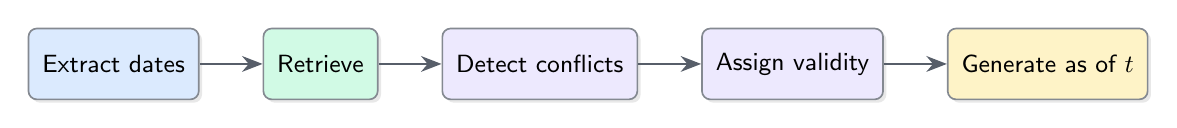
\begin{tikzpicture}[node distance=8mm]
    \node[stage=cIngest] (a) {Extract dates};
    \node[stage=cRetr, right=of a] (b) {Retrieve};
    \node[stage=cNew, right=of b] (c) {Detect conflicts};
    \node[stage=cNew, right=of c] (d) {Assign validity};
    \node[stage=cGen, right=of d] (e) {Generate as of $t$};
    \draw[arr] (a) -- (b); \draw[arr] (b) -- (c); \draw[arr] (c) -- (d); \draw[arr] (d) -- (e);
  \end{tikzpicture}
  \vspace{1.1cm}

  {\large\sffamily Major Project Final Report\par}\vspace{0.4cm}
  {\large\sffamily Submitted by: \underline{\hspace{6cm}}\par}\vspace{0.3cm}
  {\large\sffamily Roll Number: \underline{\hspace{4cm}}\par}\vspace{0.3cm}
  {\large\sffamily Guide: \underline{\hspace{6cm}}\par}\vspace{1.1cm}
  {\large\sffamily Department of Computer Science and Engineering\par}
  {\large\sffamily \underline{\hspace{8cm}}\par}
  \vfill{\sffamily November 2026\par}
\end{titlepage}

\chapter*{Abstract}
\addcontentsline{toc}{chapter}{Abstract}
Retrieval-Augmented Generation (RAG) is supposed to cure a language model's outdated knowledge, but it fails when the retrieved document is itself outdated. A September 2026 study of ``stale-document poisoning'' showed that an outdated document flips 30--37\,\% of otherwise-correct answers of open models, and up to 75\,\% when the model is told to trust the document. This project designs, implements and evaluates \textbf{TVA-RAG}, a Temporal-Validity-Aware RAG system that extracts publication and effective dates at ingestion, detects when two retrieved documents give different answers to the same question, assigns each document a validity status (CURRENT, SUPERSEDED, UNVERIFIED, FUTURE) relative to a reference date, reranks by validity, and tells the generator explicitly which evidence has expired, with an abstention path when dates cannot be verified.

Because the original study's dataset is not public, we built \textbf{TempRev}, a benchmark of 71 real-world knowledge reversals across science, software, Indian law and policy, world politics, medicine and business, each with a dated stale document and a dated current document, plus 20 stable control facts. Every reversal is queried at two reference dates: the present (gold = current answer) and a date before the change (gold = historical answer).

Across four open models served locally (llama3.2:3b, llama3.1:8b, qwen2.5:7b, qwen3.5:35b), TVA-RAG matches naive RAG when the knowledge base contains the current document (0.94 vs 0.99 pooled accuracy at the present date), is the only system that reliably answers as of a past date (0.84 pooled accuracy vs 0.34 for naive RAG, 0.37 for a recency reranker and 0.55 closed-book), and, when only the stale document exists, cuts the stale-document flip rate from 0.67--0.93 to 0.15--0.42 while converting most remaining failures into explicit abstentions. Control accuracy is unchanged at 1.00. The validity window TVA-RAG reports matches the true change date within 31 days in 72--96\,\% of cases depending on the model.

\tableofcontents
\listoffigures
\listoftables

% =====================================================================
\chapter{Introduction}
Large Language Models (LLMs) are trained on a frozen snapshot of text. RAG connects them to external documents at query time so that answers can reflect private, specialised or recently changed information. In practice a knowledge base accumulates documents over years and is rarely cleaned. A 2015 notice saying that Python~2 is supported sits next to a 2020 notice saying it has reached end of life; a 2024 circular says health insurance attracts 18\,\% GST and a September 2025 circular says it is exempt. A retriever that ranks by similarity returns both, and a generator told to ``use the documents'' may follow either.

The stale-document poisoning study \cite{stale} measured how damaging this is: models that answered correctly from their own knowledge switched to the wrong answer when handed an outdated document. The paper's own mitigation, a recency-aware reranker, reduced the effect by only 4.6--10 points. The authors observed that models followed up-to-date evidence almost perfectly, and switched almost perfectly when told \emph{when} the old evidence stopped applying. That observation is the starting point of this project: the generator does not need better reading comprehension; the system needs to tell it which evidence is still valid.

\section{Contributions}
\begin{enumerate}[leftmargin=1.6em]
  \item \textbf{TempRev}, a benchmark of 71 verified knowledge reversals with dated stale and current documents, a two-reference-date protocol, undated-document cases for abstention testing and 20 control facts.
  \item \textbf{A complete TVA-RAG implementation}: regex temporal extractor, hybrid BM25 + dense retrieval, question-conditioned claim-level conflict detector, pairwise validity status assignment, validity-aware reranking, validity prompting and abstention.
  \item \textbf{A controlled evaluation} against closed-book, naive RAG, naive RAG with a trust instruction and the recency-reranker baseline, on four open models, in a mixed-corpus and a stale-only poisoning setting (4,332 generations).
  \item \textbf{Component evaluation and ablations} of the extractor, retriever and three conflict-detector variants, a prompt ablation and an error analysis.
\end{enumerate}

% =====================================================================
\chapter{Problem Statement}
\section{Informal statement}
Given a knowledge base in which documents about the same fact were written at different times and may contradict each other, a RAG system should answer a question \emph{as it was correctly answerable on a given reference date}, cite the evidence it used, state from when that answer holds, and refuse to answer confidently when it cannot establish whether its evidence is still valid.

\section{Formal statement}
Let $D$ be a corpus of documents with unknown or partially known publication dates and possibly effective dates, $q$ a question and $t$ a reference date. Design a system $S(q,t,D)$ returning an answer $a$, cited documents $C$, a validity window $[v_{\text{from}}, v_{\text{to}})$ and an abstention flag such that:
\begin{enumerate}[label=(\alph*), leftmargin=2em]
  \item \textbf{Temporal correctness:} $a$ equals the answer that was true at time $t$.
  \item \textbf{Supersession detection:} a document whose answer has been replaced by a later document dated $\le t$ is never used as the current answer.
  \item \textbf{As-of reasoning:} documents dated after $t$ are not used.
  \item \textbf{Validity reporting:} $v_{\text{from}}$ is the date from which $a$ holds.
  \item \textbf{Calibrated abstention:} when the only relevant evidence has an unknown date and conflicts with other evidence, the system abstains.
  \item \textbf{No regression:} accuracy on questions whose answer never changed is unchanged.
\end{enumerate}
Primary metrics: temporal accuracy at $t$, stale-answer rate, stale-document flip rate, abstention rate, validity-window agreement and control accuracy.

\section{Scope}
English short-answer factual questions with one well-defined answer at any time; notice- or article-length documents; open-weight models run locally. Multi-hop temporal reasoning, multilingual documents and long documents requiring chunking are out of scope.

% =====================================================================
\chapter{Related Work}
\textbf{Stale-document poisoning.} \cite{stale} built 317 verified knowledge reversals in medicine, law, software and platform policy and tested 12 models. Outdated retrieval flipped 30\,\% of Llama and 37\,\% of Qwen answers without any trust instruction and 66--75\,\% with one; matched up-to-date evidence was followed 97--100\,\% of the time; telling the model when the old evidence stopped applying almost completely restored correctness, while a fixed recency-aware reranker reduced poisoning by only 4.6--10 points. TVA-RAG operationalises the validity-signalling finding as a system component and adds conflict detection, as-of filtering and abstention.

\textbf{Knowledge conflicts in RAG.} ConflictRAG \cite{conflictrag} detects, classifies and resolves inter-document conflicts; EvoTrustRAG \cite{evotrust} builds a conflict evidence graph with temporal relations; ArbGraph \cite{arbgraph} arbitrates claims before long-form generation; DRAGged into Conflicts \cite{dragged} gives a taxonomy of inter-context conflicts. None exposes validity windows, filters future evidence for as-of queries, or abstains on undated evidence.

\textbf{Adaptive retrieval and abstention.} Retrieval-state lock-in \cite{lockin} shows that sampling-based confidence is blind to errors caused by a stable but wrong retrieval state; Know Before You Fetch \cite{kbyf} and TARG \cite{targ} gate retrieval on calibrated uncertainty. TVA-RAG's abstention is evidence-driven rather than confidence-driven and could be combined with these.

\textbf{Temporal QA.} TimeQA \cite{timeqa}, TempLAMA \cite{templama} and SituatedQA \cite{situatedqa} study time-dependent questions for closed-book models. TempRev supplies the conflicting documents themselves so that retrieval-side handling of stale evidence can be measured.

% =====================================================================
\chapter{The TempRev Benchmark}
\section{Design}
Each reversal item records a real-world fact that changed (Table~\ref{tab:fields}); each control item is a stable fact with one dated document. Figure~\ref{fig:bench} shows how items become documents, corpus settings and queries.

\begin{table}[htbp]\centering\caption{Fields of a TempRev reversal item.}\label{tab:fields}\small
\begin{tabularx}{\linewidth}{l X}\toprule\rowcolor{cIngest}\textbf{Field}&\textbf{Description}\\\midrule
question & Present-tense factual question, e.g.\ ``What GST rate applies to individual health insurance premiums in India?''\\
old answer, aliases & Answer correct before the change, with surface variants for matching\\
new answer, aliases & Answer that became correct after the change\\
old document & Title, publication date, 40--90 word body written as a notice or article from before the change\\
new document & Title, publication date, optional effective date, body written at or after the change; most contain a supersession sentence\\
change date & Date from which the new answer holds\\
undated\_old & If true, all date cues are stripped from the stale document (7 items)\\
t\_past & Optional explicit historical reference date where an intermediate state existed\\\bottomrule\end{tabularx}\end{table}

\begin{figure}[htbp]\centering
\resizebox{\linewidth}{!}{%
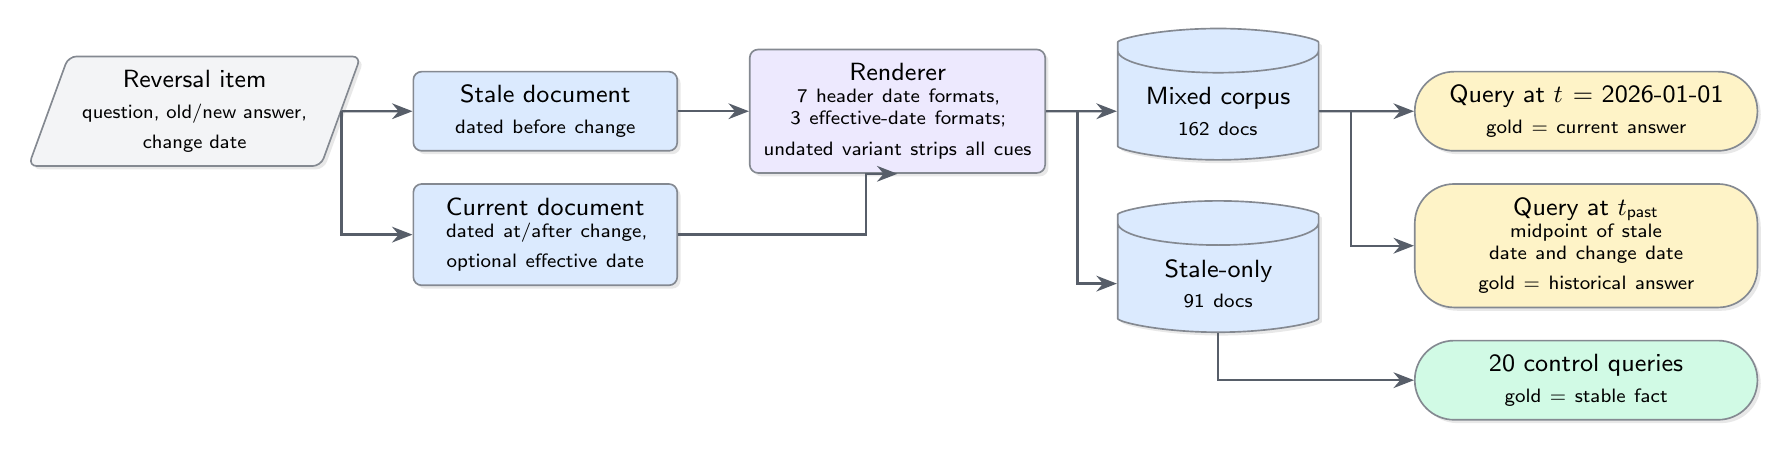
\begin{tikzpicture}[node distance=6mm and 9mm]
  \node[io] (item) {Reversal item\\\scriptsize question, old/new answer,\\\scriptsize change date};
  \node[stage=cIngest, right=of item, text width=30mm] (old) {Stale document\\\scriptsize dated before change};
  \node[stage=cIngest, below=4mm of old, text width=30mm] (new) {Current document\\\scriptsize dated at/after change,\\\scriptsize optional effective date};
  \node[stage=cNew, right=of old, text width=34mm] (render) {Renderer\\\scriptsize 7 header date formats,\\\scriptsize 3 effective-date formats;\\\scriptsize undated variant strips all cues};
  \node[store, right=of render, text width=22mm] (mixed) {Mixed corpus\\\scriptsize 162 docs};
  \node[store, below=5mm of mixed, text width=22mm] (stale) {Stale-only\\\scriptsize 91 docs};
  \node[terminal=cGen, right=12mm of mixed, text width=40mm] (qnow) {Query at $t=$ 2026-01-01\\\scriptsize gold = current answer};
  \node[terminal=cGen, below=4mm of qnow, text width=40mm] (qpast) {Query at $t_{\text{past}}$\\\scriptsize midpoint of stale date and change date\\\scriptsize gold = historical answer};
  \node[terminal=cRetr, below=4mm of qpast, text width=40mm] (qctl) {20 control queries\\\scriptsize gold = stable fact};
  \draw[arr] (item) -- (old); \draw[arr] (item.east) |- (new.west);
  \draw[arr] (old) -- (render); \draw[arr] (new.east) -| ([xshift=-4mm]render.south) -- (render.south);
  \draw[arr] (render) -- (mixed); \draw[arr] (render.east) -- ++(4mm,0) |- (stale.west);
  \draw[arr] (mixed) -- (qnow); \draw[arr] (mixed.east) -- ++(4mm,0) |- (qpast.west);
  \draw[arr] (stale.south) |- (qctl.west);
\end{tikzpicture}}
\caption{TempRev construction. 71 reversal items yield 142 dated documents and 20 controls add 20 more; two corpus settings and two reference dates give 162 (mixed) and 91 (stale-only, present date only) queries per system.}
\label{fig:bench}
\end{figure}

\section{Composition}
\begin{table}[htbp]\centering\caption{TempRev composition. Change dates range from 2006 to September 2025.}\small
\begin{tabularx}{\linewidth}{l c X}\toprule\rowcolor{cIngest}\textbf{Domain}&\textbf{Items}&\textbf{Examples}\\\midrule
Software and technology & 20 & Python 2 end of life, GitHub default branch, Java LTS, TLS 1.0/1.1, Windows 10 support, iPhone connector\\
World politics and geography & 20 & UK monarch, newest NATO member, T\"urkiye, North Macedonia, Croatia's currency, US President, Pope\\
Indian policy & 10 & Default income-tax regime, GST on online gaming, GST on health insurance, GST slabs, Union Territories, 5G, city renamings\\
Medicine and public health & 7 & COVID-19 PHEIC, USPSTF aspirin, hypertension threshold, screening ages, peanut introduction, mpox\\
Indian law & 5 & IPC to BNS, Evidence Act to BSA, Section 377, triple talaq, Article 370\\
Science & 5 & Pluto, kilogram, named elements, tallest building, Saturn's moons\\
Business & 3 & Alphabet, Twitter ownership, Air India\\
Sports & 1 & IPL team count\\\midrule
\textbf{Reversals} & \textbf{71} & 142 documents (7 stale documents rendered undated)\\
Controls & 20 & Speed of light, capital of Australia, HTTP 404, Git creator, Republic Day\\\bottomrule\end{tabularx}\end{table}

\section{Rendering and protocol}
Documents are rendered from structured fields with a header date format chosen deterministically per document from seven styles (\texttt{Published: 24 August 2006}; \texttt{Date: 2006-08-24}; \texttt{Last updated: August 2006}; \texttt{Press release dated 24/08/2006}; \texttt{Notification dated 24th August, 2006}; \texttt{(Issued 24 Aug 2006)}; \texttt{August 24, 2006}) and effective dates in three styles. Each reversal is queried at $t=$ 2026-01-01 (gold = new answer) and at $t_{\text{past}}$, the midpoint between the stale document's date and the change date (gold = old answer). The \emph{mixed} setting keeps all 162 documents; the \emph{stale-only} setting removes the 71 current documents, replicating the poisoning condition. The benchmark was authored from well-documented public facts; items should be independently verified before being cited as ground truth.

% =====================================================================
\chapter{System Architecture}
\section{Overview}
Figure~\ref{fig:arch} shows the pipeline. Offline, a temporal metadata extractor annotates every document. Online, hybrid retrieval returns five documents, a conflict detector finds pairs that answer the question differently, each document receives a validity status relative to $t$, documents are reranked by validity, and the generator receives annotated evidence with explicit rules.

\begin{figure}[htbp]\centering
\resizebox{\linewidth}{!}{%
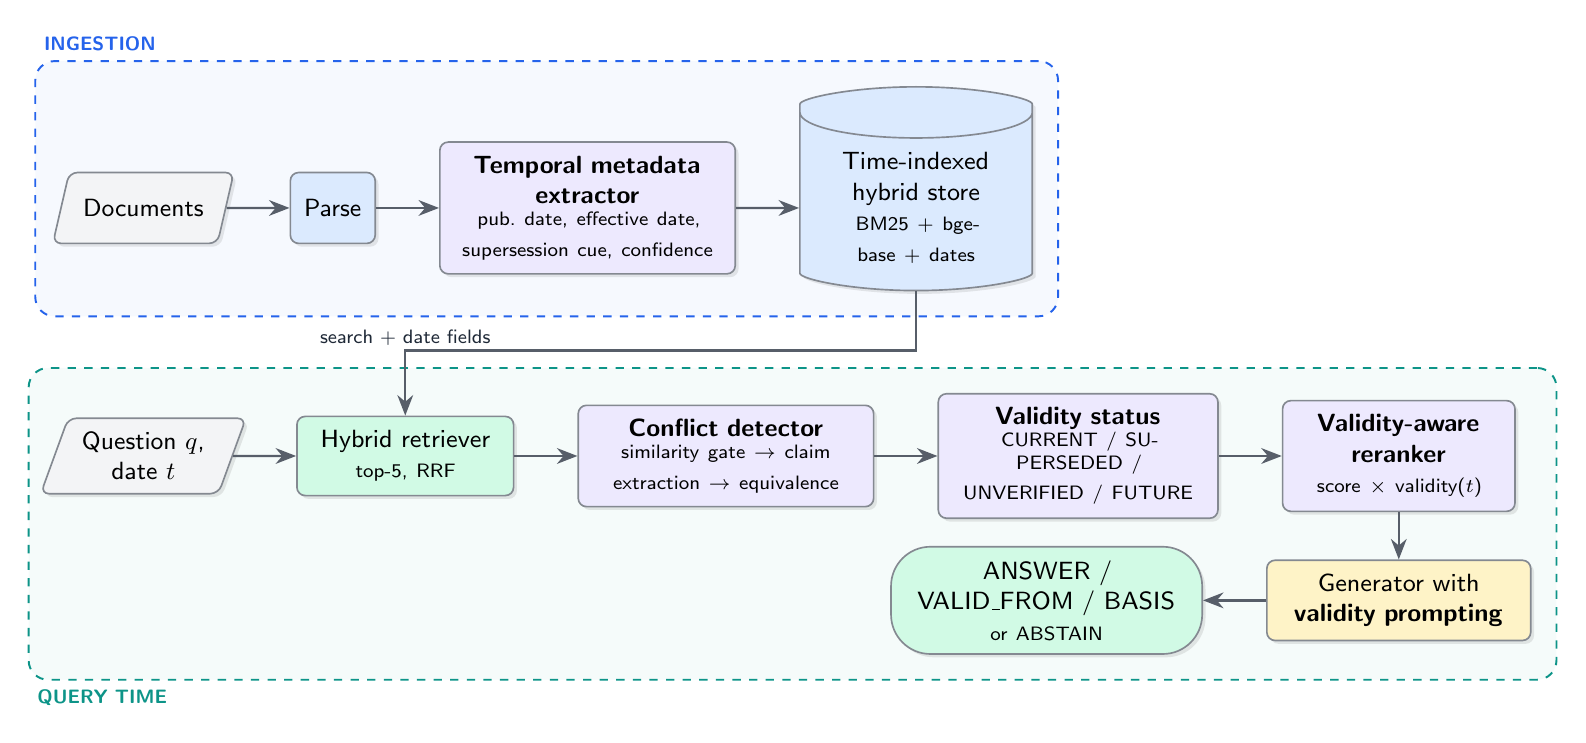
\begin{tikzpicture}[node distance=6mm and 8mm]
  \node[io] (docs) {Documents};
  \node[stage=cIngest, right=of docs] (parse) {Parse};
  \node[stage=cNew, right=of parse, text width=34mm] (tme) {\textbf{Temporal metadata}\\\textbf{extractor}\\\scriptsize pub.\ date, effective date,\\\scriptsize supersession cue, confidence};
  \node[store, right=of tme, text width=26mm] (idx) {Time-indexed\\hybrid store\\\scriptsize BM25 + bge-base + dates};
  \draw[arr] (docs) -- (parse); \draw[arr] (parse) -- (tme); \draw[arr] (tme) -- (idx);
  \node[io, below=22mm of docs] (q) {Question $q$,\\date $t$};
  \node[stage=cRetr, right=of q, text width=24mm] (ret) {Hybrid retriever\\\scriptsize top-5, RRF};
  \node[stage=cNew, right=of ret, text width=34mm] (cd) {\textbf{Conflict detector}\\\scriptsize similarity gate $\to$ claim\\\scriptsize extraction $\to$ equivalence};
  \node[stage=cNew, right=of cd, text width=32mm] (st) {\textbf{Validity status}\\\scriptsize CURRENT / SUPERSEDED /\\\scriptsize UNVERIFIED / FUTURE};
  \node[stage=cNew, right=of st, text width=26mm] (rr) {\textbf{Validity-aware}\\\textbf{reranker}\\\scriptsize score $\times$ validity($t$)};
  \node[stage=cGen, below=of rr, text width=30mm] (gen) {Generator with\\\textbf{validity prompting}};
  \node[terminal=cRetr, left=of gen, text width=36mm] (out) {ANSWER / VALID\_FROM / BASIS\\\scriptsize or ABSTAIN};
  \draw[arr] (q) -- (ret); \draw[arr] (ret) -- (cd); \draw[arr] (cd) -- (st); \draw[arr] (st) -- (rr); \draw[arr] (rr) -- (gen); \draw[arr] (gen) -- (out);
  \draw[arr] (idx.south) -- ++(0,-7.5mm) -| node[lbl,pos=0.5,above]{search + date fields} (ret.north);
  \begin{scope}[on background layer]
    \node[group=accent, fit=(docs)(parse)(tme)(idx)] (g1) {}; \node[glabel=accent] at (g1.north west) {INGESTION};
    \node[group=teal, fit=(q)(ret)(cd)(st)(rr)(gen)(out)] (g2) {}; \node[glabel=teal, anchor=north west] at (g2.south west) {QUERY TIME};
  \end{scope}
\end{tikzpicture}}
\caption{TVA-RAG architecture. Purple components are additions to an advanced RAG pipeline.}
\label{fig:arch}
\end{figure}

\section{Temporal metadata extractor}
A regex extractor recognises ISO dates, day-month-year and month-day-year forms with ordinal suffixes, numeric \texttt{dd/mm/yyyy}, \texttt{dd-mm-yyyy} and \texttt{dd.mm.yyyy}, and month-year forms (month precision). The publication date is the first date in the first three lines (confidence 0.95 at day precision, 0.8 at month precision), else the first date in the body (0.5). The effective date is a date within 40 characters after a cue such as \emph{effective from}, \emph{with effect from}, \emph{w.e.f.}, \emph{comes into force}. A supersession cue flag is set by words such as \emph{supersedes}, \emph{replaces}, \emph{no longer}, \emph{repeal}, \emph{retired}, \emph{renamed}. The \emph{anchor} used for validity reasoning is the effective date if present, else the publication date. An optional LLM fallback is invoked only when no date is found and is instructed not to infer dates from historical content.

\section{Hybrid retriever}
BM25 over lowercased tokens and dense retrieval with BAAI/bge-base-en-v1.5 are fused with reciprocal rank fusion ($k=60$); the top five documents are passed on.

\section{Conflict detector}
Figure~\ref{fig:detector} shows the question-conditioned claim detector. Candidates pass a similarity gate (whole-text embedding similarity $\ge 0.60$ with at least one other retrieved document; on TempRev no true conflicting pair falls below 0.70). A detector LLM (qwen3.5:35b) states the shortest answer each candidate gives to the exact question, or NONE after a scope check. Two documents conflict when both give an answer and the answers are not identical after normalisation and the detector LLM judges them different (different names or spellings, entities, numbers, versions, dates, or opposite yes/no). All calls are cached per (question, document) and shared across generator models. An NLI variant (cross-encoder, similarity-gated) is kept as an ablation.

\begin{figure}[htbp]\centering
\resizebox{\linewidth}{!}{%
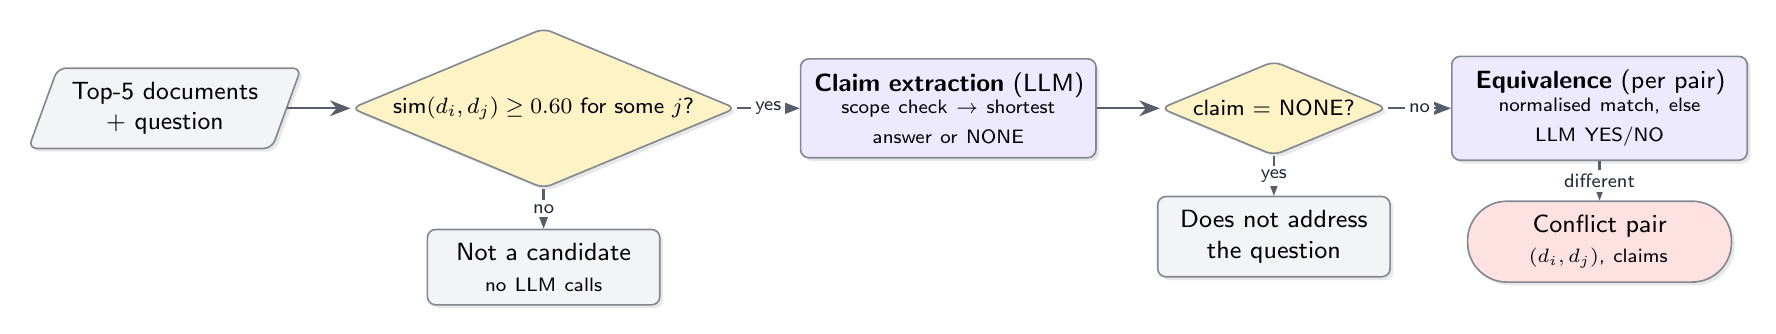
\begin{tikzpicture}[node distance=5mm and 8mm]
  \node[io] (in) {Top-5 documents\\+ question};
  \node[decision, right=of in] (gate) {sim$(d_i,d_j)\ge 0.60$ for some $j$?};
  \node[stage=cGray, below=of gate, text width=26mm] (skip) {Not a candidate\\\scriptsize no LLM calls};
  \node[stage=cNew, right=of gate, text width=34mm] (claim) {\textbf{Claim extraction} (LLM)\\\scriptsize scope check $\to$ shortest\\\scriptsize answer or NONE};
  \node[decision, right=of claim] (none) {claim = NONE?};
  \node[stage=cGray, below=of none, text width=26mm] (drop) {Does not address\\the question};
  \node[stage=cNew, right=of none, text width=34mm] (eq) {\textbf{Equivalence} (per pair)\\\scriptsize normalised match, else\\\scriptsize LLM YES/NO};
  \node[terminal=cSec, below=of eq, text width=30mm] (conf) {Conflict pair\\\scriptsize $(d_i, d_j)$, claims};
  \draw[arr] (in) -- (gate); \draw[arr] (gate) -- node[lbl]{no} (skip); \draw[arr] (gate) -- node[lbl]{yes} (claim);
  \draw[arr] (claim) -- (none); \draw[arr] (none) -- node[lbl]{yes} (drop); \draw[arr] (none) -- node[lbl]{no} (eq);
  \draw[arr] (eq) -- node[lbl]{different} (conf);
\end{tikzpicture}}
\caption{Question-conditioned claim-level conflict detection.}
\label{fig:detector}
\end{figure}

\section{Validity status assignment}
Status is assigned pairwise rather than through transitive clusters, so a single false conflict cannot drag unrelated documents into one cluster (Figure~\ref{fig:status}, Table~\ref{tab:status}). Dropping FUTURE documents is what makes as-of answers possible: at a past reference date the current document is simply not shown.

\begin{table}[htbp]\centering\caption{Validity statuses relative to the reference date $t$.}\label{tab:status}\small
\begin{tabularx}{\linewidth}{l X c}\toprule\rowcolor{cIngest}\textbf{Status}&\textbf{Condition}&\textbf{Validity}\\\midrule
FUTURE & anchor date $> t$ & 0 (dropped)\\
SUPERSEDED & conflicts with a non-future document whose anchor is later; records \emph{superseded\_by}, \emph{superseded\_on} & 0.25\\
CURRENT & conflicts with others and none is later & 1.0\\
UNVERIFIED & no date could be established & 0.6 (0.4 if conflicting)\\
UNCONFLICTED & dated, no conflicts & 1.0\\\bottomrule\end{tabularx}\end{table}

\begin{figure}[htbp]\centering
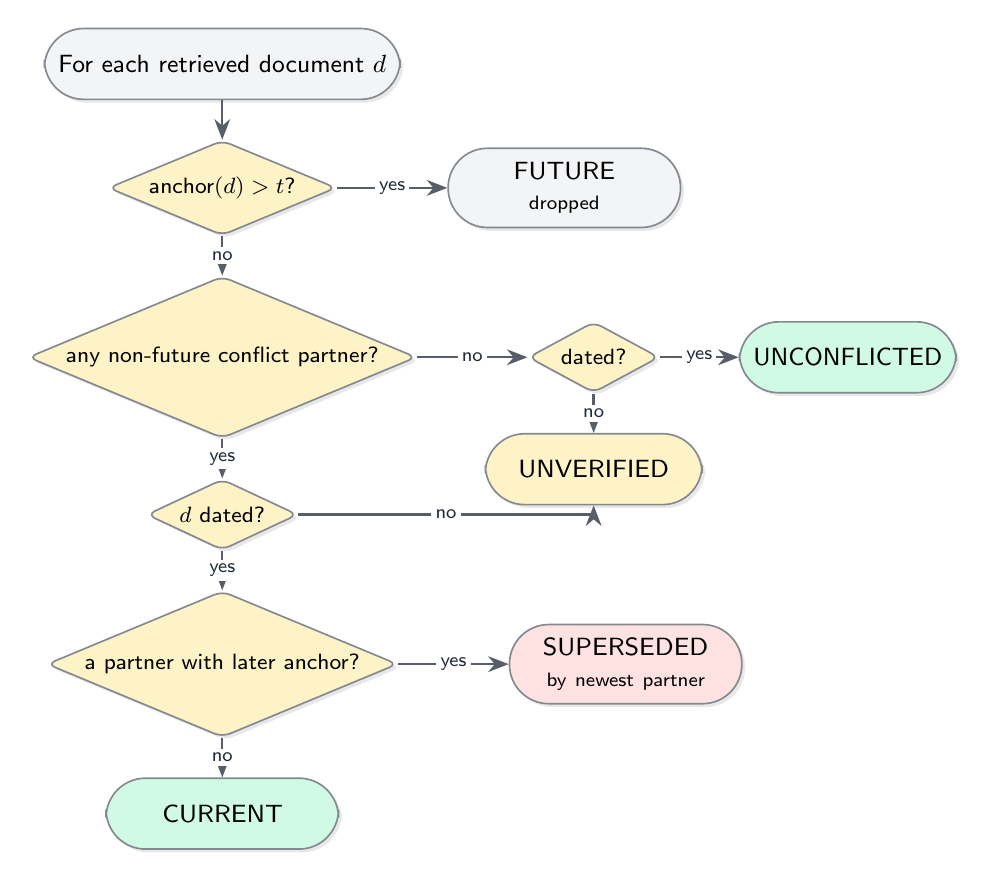
\begin{tikzpicture}[node distance=5mm and 12mm]
  \node[terminal=cGray] (s) {For each retrieved document $d$};
  \node[decision, below=of s] (d1) {anchor$(d) > t$?};
  \node[terminal=cGray, right=14mm of d1, text width=26mm] (fut) {FUTURE\\\scriptsize dropped};
  \node[decision, below=of d1] (d2) {any non-future conflict partner?};
  \node[decision, right=14mm of d2] (d3) {dated?};
  \node[terminal=cRetr, right=10mm of d3, text width=24mm] (unc) {UNCONFLICTED};
  \node[terminal=cGen, below=of d3, text width=24mm] (unv) {UNVERIFIED};
  \node[decision, below=of d2] (d4) {$d$ dated?};
  \node[decision, below=of d4] (d5) {a partner with later anchor?};
  \node[terminal=cSec, right=14mm of d5, text width=26mm] (sup) {SUPERSEDED\\\scriptsize by newest partner};
  \node[terminal=cRetr, below=of d5, text width=26mm] (cur) {CURRENT};
  \draw[arr] (s) -- (d1); \draw[arr] (d1) -- node[lbl]{yes} (fut); \draw[arr] (d1) -- node[lbl]{no} (d2);
  \draw[arr] (d2) -- node[lbl]{no} (d3); \draw[arr] (d3) -- node[lbl]{yes} (unc); \draw[arr] (d3) -- node[lbl]{no} (unv);
  \draw[arr] (d2) -- node[lbl]{yes} (d4); \draw[arr] (d4.east) -| node[lbl,pos=0.25]{no} (unv.south);
  \draw[arr] (d4) -- node[lbl]{yes} (d5); \draw[arr] (d5) -- node[lbl]{yes} (sup); \draw[arr] (d5) -- node[lbl]{no} (cur);
\end{tikzpicture}
\caption{Pairwise validity status assignment.}
\label{fig:status}
\end{figure}

\section{Reranker, validity prompting and abstention}
$\text{final\_score} = \text{retrieval\_score} \times \text{validity} \times \text{source\_trust}$; superseded documents stay in context but sink below current ones. Each document is presented as \texttt{[Document i | dated: d | status: ...]} with the reference date and rules: prefer CURRENT evidence; never return a SUPERSEDED answer as current; do not abstain when a CURRENT document answers; answer ABSTAIN only when no CURRENT document answers and the only relevant evidence is DATE UNKNOWN and conflicting; output \texttt{ANSWER}, \texttt{VALID\_FROM}, \texttt{BASIS}. In the stale-only setting the document's age at $t$ is stated and the model is told not to assume a time-varying fact is still valid, to use its own knowledge if confident, and otherwise to abstain (full prompts in Appendix~\ref{app:prompts}).

\section{Baselines}
\begin{table}[htbp]\centering\caption{Systems compared. All receive the reference date.}\small
\begin{tabularx}{\linewidth}{l X}\toprule\rowcolor{cIngest}\textbf{Mode}&\textbf{Description}\\\midrule
closed\_book & No retrieval\\
naive & Hybrid top-5, raw documents (dates visible in text)\\
naive\_trust & naive + ``your answer must follow the information in the documents'' (the poisoning paper's trust condition)\\
recency & Top-5 ordered newest first by extracted anchor date; no status annotation (the poisoning paper's reranker baseline)\\
tva & Full TVA-RAG\\\bottomrule\end{tabularx}\end{table}

% =====================================================================
\chapter{Implementation and Experimental Setup}
\section{Implementation}
The system is a Python package (\texttt{tva\_rag/src/tva\_rag}: \texttt{corpus}, \texttt{temporal}, \texttt{retriever}, \texttt{conflict}, \texttt{reranker}, \texttt{generator}, \texttt{judge}, \texttt{pipeline}) with a benchmark builder, a resumable grid runner, an analysis script and a Streamlit demo. Stack: Python 3.14, PyTorch 2.14 (CUDA), sentence-transformers 6.2, rank\_bm25, pandas, matplotlib, Ollama 0.31. Hardware: one NVIDIA RTX PRO 5000 (48\,GB), 123\,GB RAM. Generators: llama3.2:3b, llama3.1:8b, qwen2.5:7b, qwen3.5:35b (thinking disabled); detector and judge: qwen3.5:35b; embeddings: bge-base-en-v1.5; NLI ablation: nli-deberta-v3-base. Generation uses temperature 0, a fixed seed, a 6,144-token context and at most 220 output tokens. The Ollama client retries with back-off, the runner resumes by record key, and every detector and judge call is cached on disk.

\section{Experimental grid}
\begin{figure}[htbp]\centering
\resizebox{\linewidth}{!}{%
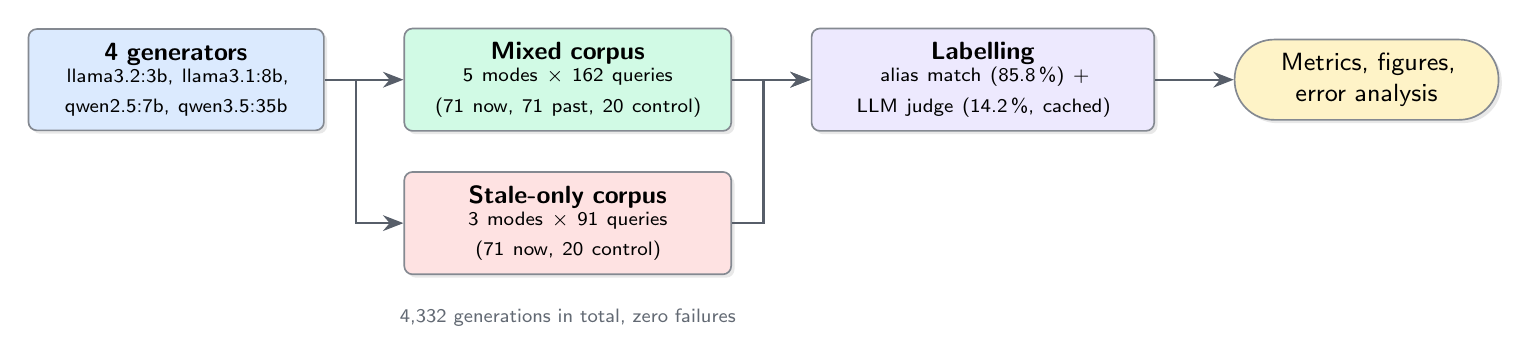
\begin{tikzpicture}[node distance=5mm and 10mm]
  \node[stage=cIngest, text width=34mm] (models) {\textbf{4 generators}\\\scriptsize llama3.2:3b, llama3.1:8b,\\\scriptsize qwen2.5:7b, qwen3.5:35b};
  \node[stage=cRetr, right=of models, text width=38mm] (mixed) {\textbf{Mixed corpus}\\\scriptsize 5 modes $\times$ 162 queries\\\scriptsize (71 now, 71 past, 20 control)};
  \node[stage=cSec, below=of mixed, text width=38mm] (stale) {\textbf{Stale-only corpus}\\\scriptsize 3 modes $\times$ 91 queries\\\scriptsize (71 now, 20 control)};
  \node[stage=cNew, right=of mixed, text width=40mm] (label) {\textbf{Labelling}\\\scriptsize alias match (85.8\,\%) +\\\scriptsize LLM judge (14.2\,\%, cached)};
  \node[terminal=cGen, right=of label, text width=30mm] (met) {Metrics, figures,\\error analysis};
  \draw[arr] (models) -- (mixed); \draw[arr] (models.east) -- ++(4mm,0) |- (stale.west);
  \draw[arr] (mixed) -- (label); \draw[arr] (stale.east) -- ++(4mm,0) |- (label.west); \draw[arr] (label) -- (met);
  \node[font=\scriptsize\sffamily, below=3mm of stale, text=ink!70] {4,332 generations in total, zero failures};
\end{tikzpicture}}
\caption{Experimental design.}
\end{figure}

\section{Metrics}
\emph{Accuracy at $t$} (label equals gold); \emph{stale-answer rate} (OLD when gold is NEW); \emph{flip rate} (among items answered correctly closed-book at $t=$ now, fraction answered OLD under a RAG mode, the poisoning paper's metric); \emph{abstention rate}; \emph{validity window} (whether \texttt{VALID\_FROM} is stated and within 31 days or one year of the true change date); component metrics (extractor anchor accuracy, retrieval recall@5, detector pair precision/recall on on-topic pairs, status correctness).

\section{Prompt refinement}
A pilot run revealed that qwen2.5:7b abstained in 15.5\,\% of present-date queries even with a CURRENT document available and that the 3B model sometimes wrote the status word CURRENT as its answer. The TVA instruction was clarified and TVA mode rerun for all models; baselines were not changed and both TVA versions are reported (Section~\ref{sec:promptabl}).

% =====================================================================
\chapter{Results}
\section{Mixed corpus, present reference date}
\begin{table}[htbp]\centering\caption{Accuracy at $t=$ 2026-01-01, mixed corpus (stale-answer rate in brackets; last column = TVA-RAG abstention rate).}
\label{tab:now}\footnotesize\setlength{\tabcolsep}{4pt}
\begin{tabular}{l c c c c c c}\toprule\rowcolor{cIngest}\textbf{Model}&\textbf{Closed-book}&\textbf{Naive}&\textbf{Naive+trust}&\textbf{Recency}&\textbf{TVA-RAG}&\textbf{TVA abst.}\\\midrule
llama3.2:3b & 0.606 (0.155) & 0.972 (0.028) & 0.972 (0.028) & 0.887 (0.113) & 0.944 (0.042) & 0.014\\
llama3.1:8b & 0.690 (0.239) & 0.986 (0.014) & 0.986 (0.014) & 0.958 (0.042) & \textbf{0.986} (0.000) & 0.014\\
qwen2.5:7b  & 0.634 (0.211) & 1.000 (0.000) & 1.000 (0.000) & 0.944 (0.056) & 0.845 (0.014) & 0.141\\
qwen3.5:35b & 0.775 (0.197) & 0.986 (0.000) & 0.986 (0.014) & 1.000 (0.000) & 0.986 (0.000) & 0.014\\\midrule
\rowcolor{cNew}\textbf{Pooled} & 0.676 (0.201) & \textbf{0.986} (0.011) & 0.986 (0.014) & 0.947 (0.053) & 0.940 (0.014) & 0.046\\\bottomrule\end{tabular}
\end{table}

\begin{figure}[htbp]\centering
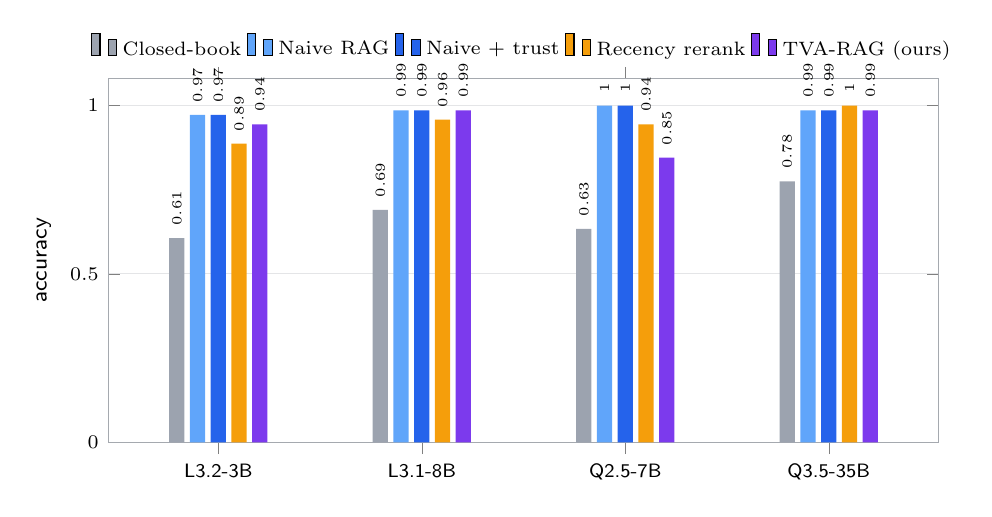
\begin{tikzpicture}
\begin{axis}[resbar, legend entries={Closed-book, Naive RAG, Naive + trust, Recency rerank, TVA-RAG (ours)}]
\addplot[fill=bCB, draw=none] coordinates {(L3.2-3B,0.606) (L3.1-8B,0.690) (Q2.5-7B,0.634) (Q3.5-35B,0.775)};
\addplot[fill=bNaive, draw=none] coordinates {(L3.2-3B,0.972) (L3.1-8B,0.986) (Q2.5-7B,1.000) (Q3.5-35B,0.986)};
\addplot[fill=bTrust, draw=none] coordinates {(L3.2-3B,0.972) (L3.1-8B,0.986) (Q2.5-7B,1.000) (Q3.5-35B,0.986)};
\addplot[fill=bRec, draw=none] coordinates {(L3.2-3B,0.887) (L3.1-8B,0.958) (Q2.5-7B,0.944) (Q3.5-35B,1.000)};
\addplot[fill=bTVA, draw=none] coordinates {(L3.2-3B,0.944) (L3.1-8B,0.986) (Q2.5-7B,0.845) (Q3.5-35B,0.986)};
\end{axis}
\end{tikzpicture}
\caption{Accuracy on reversal questions at the present reference date (gold = current answer), mixed corpus.}
\end{figure}

When the current document is in the knowledge base, naive RAG is already near the ceiling: all four models prefer the document that answers the question most directly, and most current documents carry a supersession sentence. TVA-RAG matches naive RAG for llama3.1:8b and qwen3.5:35b; its pooled gap of 4.6 points is almost entirely qwen2.5:7b's abstentions (10 of 71, all with a CURRENT document present). TVA-RAG has the lowest stale-answer rate of the retrieval modes for three of four models. The recency reranker is \emph{worse} than naive RAG for three models (pooled stale-answer rate 0.053 vs 0.011): newest-first ordering puts recent documents about other topics first and the model over-weights ``Document~1''.

\section{Mixed corpus, past reference date}
\begin{table}[htbp]\centering\caption{Accuracy at $t_{\text{past}}$ (gold = historical answer), mixed corpus.}\label{tab:past}\small
\begin{tabularx}{\linewidth}{l c c c c X}\toprule\rowcolor{cIngest}\textbf{Model}&\textbf{Closed-book}&\textbf{Naive}&\textbf{Naive+trust}&\textbf{Recency}&\textbf{TVA-RAG}\\\midrule
llama3.2:3b & 0.465 & 0.085 & 0.127 & 0.169 & \textbf{0.732}\\
llama3.1:8b & 0.577 & 0.437 & 0.352 & 0.423 & \textbf{0.972}\\
qwen2.5:7b  & 0.394 & 0.028 & 0.000 & 0.099 & \textbf{0.775} (abst 0.169)\\
qwen3.5:35b & 0.761 & 0.817 & 0.535 & 0.789 & \textbf{0.873} (abst 0.127)\\\midrule
\rowcolor{cNew}\textbf{Pooled} & 0.549 & 0.342 & 0.254 & 0.370 & \textbf{0.838} (abst 0.074)\\\bottomrule\end{tabularx}\end{table}

\begin{figure}[htbp]\centering
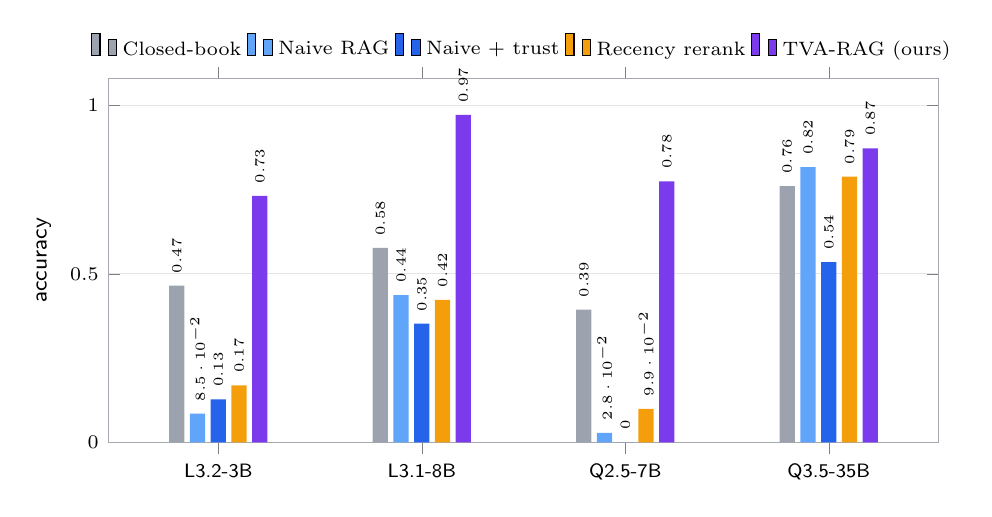
\begin{tikzpicture}
\begin{axis}[resbar, legend entries={Closed-book, Naive RAG, Naive + trust, Recency rerank, TVA-RAG (ours)}]
\addplot[fill=bCB, draw=none] coordinates {(L3.2-3B,0.465) (L3.1-8B,0.577) (Q2.5-7B,0.394) (Q3.5-35B,0.761)};
\addplot[fill=bNaive, draw=none] coordinates {(L3.2-3B,0.085) (L3.1-8B,0.437) (Q2.5-7B,0.028) (Q3.5-35B,0.817)};
\addplot[fill=bTrust, draw=none] coordinates {(L3.2-3B,0.127) (L3.1-8B,0.352) (Q2.5-7B,0.000) (Q3.5-35B,0.535)};
\addplot[fill=bRec, draw=none] coordinates {(L3.2-3B,0.169) (L3.1-8B,0.423) (Q2.5-7B,0.099) (Q3.5-35B,0.789)};
\addplot[fill=bTVA, draw=none] coordinates {(L3.2-3B,0.732) (L3.1-8B,0.972) (Q2.5-7B,0.775) (Q3.5-35B,0.873)};
\end{axis}
\end{tikzpicture}
\caption{Accuracy on reversal questions at a reference date before the change (gold = historical answer).}
\end{figure}

This is the setting where temporal reasoning is unavoidable. Although every baseline is told the reference date, naive RAG answers with the \emph{current} fact in 182 of 187 wrong cases. Retrieval makes the smaller models worse than closed-book (llama3.2:3b 0.465 $\to$ 0.085; qwen2.5:7b 0.394 $\to$ 0.028). TVA-RAG, by dropping FUTURE documents and labelling the rest, raises pooled accuracy from 0.342 to 0.838 and reaches 0.972 with llama3.1:8b. Only the 35B model can partially reason about dates by itself.

\section{Control questions}
All retrieval modes score 1.000 on the 20 control questions for all four models (closed-book 0.85--1.00). TVA-RAG causes no regression on stable facts.

\section{Stale-only corpus: poisoning replication}
\begin{table}[htbp]\centering\caption{Stale-only corpus, $t=$ 2026-01-01: only the stale document exists (naive / naive+trust / TVA-RAG).}\label{tab:stale}\footnotesize
\begin{tabular}{l c c c}\toprule\rowcolor{cIngest}\textbf{Model}&\textbf{Accuracy}&\textbf{Stale-answer rate}&\textbf{Abstention}\\\midrule
llama3.2:3b & 0.225 / 0.169 / \textbf{0.366} & 0.732 / 0.761 / \textbf{0.535} & 0 / 0 / 0.070\\
llama3.1:8b & 0.099 / 0.113 / \textbf{0.268} & 0.845 / 0.845 / \textbf{0.352} & 0 / 0 / 0.366\\
qwen2.5:7b  & 0.056 / 0.056 / \textbf{0.113} & 0.930 / 0.930 / \textbf{0.549} & 0 / 0 / 0.338\\
qwen3.5:35b & 0.028 / 0.028 / \textbf{0.465} & 0.915 / 0.930 / \textbf{0.310} & 0 / 0 / 0.225\\\midrule
\rowcolor{cNew}\textbf{Pooled} & 0.102 / 0.092 / \textbf{0.303} & 0.856 / 0.866 / \textbf{0.437} & 0 / 0 / 0.250\\\bottomrule\end{tabular}\end{table}

\begin{table}[htbp]\centering\caption{Flip rate: among items answered correctly closed-book, fraction flipped to the stale answer (stale-only corpus).}\label{tab:flip}\small
\begin{tabularx}{\linewidth}{l c c c X c c}\toprule\rowcolor{cIngest}\textbf{Model}&\textbf{$n$}&\textbf{Naive}&\textbf{Naive+trust}&\textbf{TVA-RAG}&\textbf{TVA abstains}&\textbf{TVA still correct}\\\midrule
llama3.2:3b & 43 & 0.674 & 0.698 & \textbf{0.419} & 0.070 & 0.512\\
llama3.1:8b & 49 & 0.776 & 0.776 & \textbf{0.204} & 0.388 & 0.388\\
qwen2.5:7b  & 45 & 0.889 & 0.889 & \textbf{0.378} & 0.467 & 0.156\\
qwen3.5:35b & 55 & 0.909 & 0.927 & \textbf{0.145} & 0.255 & 0.600\\\bottomrule\end{tabularx}\end{table}

\begin{figure}[htbp]\centering
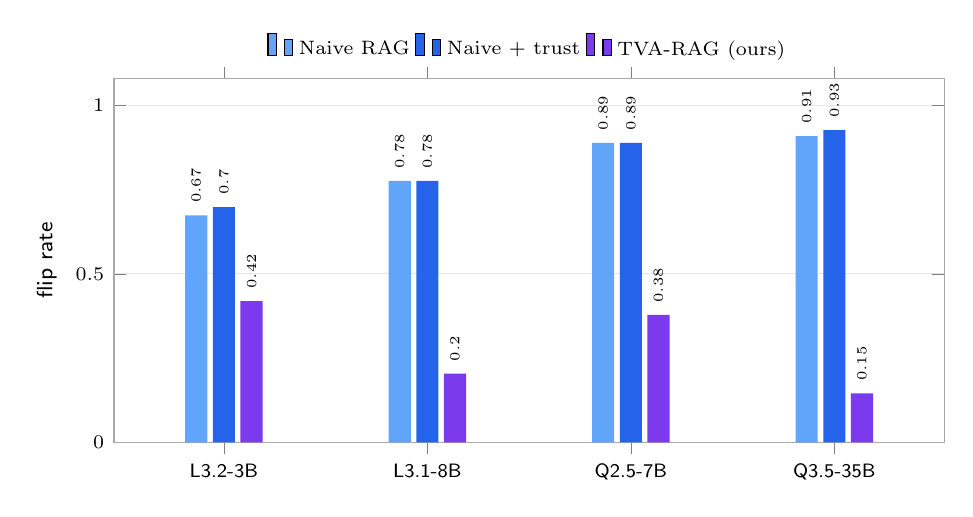
\begin{tikzpicture}
\begin{axis}[resbar, ylabel={flip rate}, bar width=8pt, legend entries={Naive RAG, Naive + trust, TVA-RAG (ours)}, legend columns=3]
\addplot[fill=bNaive, draw=none] coordinates {(L3.2-3B,0.674) (L3.1-8B,0.776) (Q2.5-7B,0.889) (Q3.5-35B,0.909)};
\addplot[fill=bTrust, draw=none] coordinates {(L3.2-3B,0.698) (L3.1-8B,0.776) (Q2.5-7B,0.889) (Q3.5-35B,0.927)};
\addplot[fill=bTVA, draw=none] coordinates {(L3.2-3B,0.419) (L3.1-8B,0.204) (Q2.5-7B,0.378) (Q3.5-35B,0.145)};
\end{axis}
\end{tikzpicture}
\caption{Stale-document poisoning: fraction of closed-book-correct answers flipped to the stale answer.}
\end{figure}

Our naive flip rates (0.67--0.91) exceed the 30--37\,\% of \cite{stale} because TempRev's stale documents answer the question directly and the models are small. TVA-RAG's age signalling and abstention rule reduce the flip rate by 26--76 points; qwen3.5:35b keeps 60\,\% of its correct closed-book answers (vs 4\,\% with naive RAG) and abstains on another 26\,\%. In the mixed setting all RAG modes have flip rates below 0.10 and TVA-RAG has zero flips for llama3.1:8b and qwen3.5:35b.

\section{Validity-window reporting and latency}
\begin{table}[htbp]\centering\caption{TVA-RAG validity window at the present date.}\small
\begin{tabular}{l c c c}\toprule\rowcolor{cIngest}\textbf{Model}&\textbf{VALID\_FROM stated}&\textbf{Within 31 days of change}&\textbf{Within 1 year}\\\midrule
llama3.2:3b & 1.000 & 0.873 & 0.901\\ llama3.1:8b & 0.986 & 0.944 & 0.958\\ qwen2.5:7b & 0.915 & 0.718 & 0.775\\ qwen3.5:35b & 0.986 & 0.958 & 0.972\\\bottomrule\end{tabular}\end{table}
Mean per-query latency (mixed corpus, detector cached): closed-book 0.46\,s, naive 0.49\,s, recency 0.48\,s, TVA 0.74\,s. Uncached detection with qwen3.5:35b costs about 1.7\,s per query; with the NLI detector 0.06\,s.

\section{Qualitative example}
Question: \emph{What GST rate applies to individual health insurance premiums in India?} (llama3.1:8b).
\begin{table}[htbp]\centering\small
\begin{tabularx}{\linewidth}{l X}\toprule\rowcolor{cIngest}\textbf{Mode, date}&\textbf{Output}\\\midrule
naive, 2026-01-01 & ``As per Document 2, dated September 22, 2025, individual health insurance policies are exempt from GST. ANSWER: Exempt.''\\
naive, 2024-11-28 & ``As per Document 2 dated September 22, 2025, individual health insurance policies are now exempt from GST. ANSWER: Exempt.'' (wrong: the exemption was ten months in the future)\\
TVA, 2026-01-01 & ``ANSWER: Exempt / VALID\_FROM: 2025-09-22 / BASIS: Document 1''\\
TVA, 2024-11-28 & ``ANSWER: 18\% / VALID\_FROM: 2024-02-05 / BASIS: Document 1'' (the 2025 document was FUTURE and dropped)\\\bottomrule\end{tabularx}\end{table}

% =====================================================================
\chapter{Component Evaluation and Ablations}
\section{Extractor and retriever}
\begin{table}[htbp]\centering\caption{Component metrics.}\small
\begin{tabularx}{\linewidth}{X c c}\toprule\rowcolor{cIngest}\textbf{Metric}&\textbf{Value}&\textbf{$n$}\\\midrule
Extractor anchor-date accuracy, regex (all documents, seven header formats) & 1.000 & 162\\
Extractor reports ``unknown'' on undated documents & 1.000 & 7\\
LLM fallback hallucinates a date on undated documents & 0.000 & 7\\
Retrieval recall@5 of both item documents: BM25 / dense / hybrid & 0.944 / 1.000 / 0.986 & 71\\
Deployed detector across the full run: pair precision / recall / F1 & 0.922 / 0.757 / 0.831 & 149\\
Items' own documents receiving the correct status & 0.848 & 211\\\bottomrule\end{tabularx}\end{table}
Retrieval is not the bottleneck: both conflicting documents are almost always in the top five, which is exactly what makes stale evidence a problem.

\section{Conflict detector variants}
\begin{table}[htbp]\centering\caption{Detector variants on on-topic retrieved pairs (71 present-date questions).}\label{tab:det}\small
\begin{tabular}{l c c c l}\toprule\rowcolor{cIngest}\textbf{Detector}&\textbf{Precision}&\textbf{Recall}&\textbf{F1}&\textbf{Cost / query}\\\midrule
\rowcolor{cNew}\textbf{Claims, qwen3.5:35b (used)} & \textbf{0.898} & 0.757 & \textbf{0.822} & 1.7\,s uncached\\
NLI cross-encoder, similarity-gated & 0.727 & \textbf{0.914} & 0.810 & 0.06\,s\\
Claims, llama3.1:8b & 0.549 & 0.800 & 0.651 & 1.1\,s\\\bottomrule\end{tabular}\end{table}

\begin{figure}[htbp]\centering
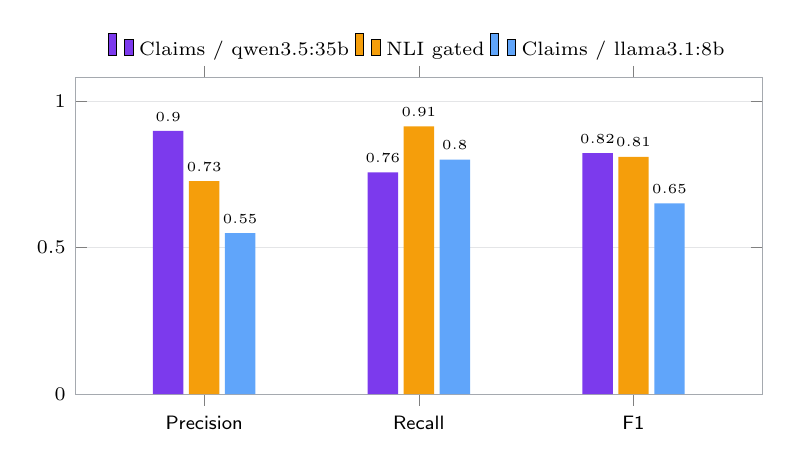
\begin{tikzpicture}
\begin{axis}[ybar, width=0.85\linewidth, height=5.6cm, ymin=0, ymax=1.08, symbolic x coords={Precision,Recall,F1}, xtick=data, enlarge x limits=0.3, bar width=11pt,
  legend style={font=\scriptsize, draw=none, fill=none, at={(0.5,1.02)}, anchor=south, legend columns=3}, tick label style={font=\scriptsize\sffamily},
  ymajorgrids, grid style={ink!12}, axis line style={ink!40}, nodes near coords, every node near coord/.append style={font=\tiny},
  legend entries={Claims / qwen3.5:35b, NLI gated, Claims / llama3.1:8b}]
\addplot[fill=bTVA, draw=none] coordinates {(Precision,0.898) (Recall,0.757) (F1,0.822)};
\addplot[fill=bRec, draw=none] coordinates {(Precision,0.727) (Recall,0.914) (F1,0.810)};
\addplot[fill=bNaive, draw=none] coordinates {(Precision,0.549) (Recall,0.800) (F1,0.651)};
\end{axis}
\end{tikzpicture}
\caption{Conflict detector variants.}
\end{figure}

Precision was deliberately favoured: a false conflict can mark the correct document SUPERSEDED, whereas a missed conflict only degrades TVA-RAG to naive behaviour for that query. The NLI model alone was unusable (median contradiction probability 0.99 on \emph{unrelated} pairs, 0.003 on a genuine mammography 50-vs-40 conflict) and works only behind a similarity gate; the 8B model extracted claims adequately but judged ``main'' and ``master'' to be the same answer. At the present date 76\,\% of current documents were marked CURRENT, 68\,\% of stale documents SUPERSEDED, 10\,\% UNVERIFIED (the undated ones), and 1.4\,\% of current documents were wrongly SUPERSEDED.

\section{Prompt ablation}\label{sec:promptabl}
\begin{table}[htbp]\centering\caption{Pilot vs final TVA instruction (accuracy).}\small
\begin{tabular}{l c c c c}\toprule\rowcolor{cIngest}\textbf{Metric}&\textbf{llama3.2:3b}&\textbf{llama3.1:8b}&\textbf{qwen2.5:7b}&\textbf{qwen3.5:35b}\\\midrule
$t=$ now, pilot & 0.958 & 0.972 & 0.831 (abst 0.155) & 1.000\\
$t=$ now, final & 0.944 & 0.986 & 0.845 (abst 0.141) & 0.986\\
$t_{\text{past}}$, pilot & 0.718 & 0.817 & 0.704 & 0.873\\
$t_{\text{past}}$, final & 0.732 & 0.972 & 0.775 & 0.873\\
stale-only, pilot & 0.380 & 0.254 & 0.113 & 0.465\\
stale-only, final & 0.366 & 0.268 & 0.113 & 0.465\\\bottomrule\end{tabular}\end{table}
Clarifying the abstention rule helped llama3.1:8b substantially at the past date and barely moved the others; qwen2.5:7b's over-abstention is a model trait.

% =====================================================================
\chapter{Error Analysis and Discussion}
\section{Error analysis}
\begin{itemize}[leftmargin=1.4em]
  \item \textbf{TVA-RAG at the present date (4 non-abstaining errors of 284).} llama3.2:3b answered ``No'' to the triple-talaq and 5G questions and ``Joe Biden'' for the US President despite a CURRENT document saying otherwise (parametric prior wins over the annotation); qwen2.5:7b answered ``Croatian kuna (SUPERSEDED)'', echoing the status label.
  \item \textbf{qwen2.5:7b abstentions (10 of 71).} All had a CURRENT document; seven were software lifecycle yes/no questions. The model treats any SUPERSEDED or DATE UNKNOWN document as grounds to abstain, contrary to the instruction. A deterministic post-check that overrides ABSTAIN when a CURRENT document carries a claim would remove most of these.
  \item \textbf{TVA-RAG at the past date (46 errors of 284).} llama3.2:3b: 15 current-fact answers (parametric leakage after the current document was dropped as FUTURE) and 4 malformed; qwen2.5:7b: 12 abstentions, 4 current-fact answers; qwen3.5:35b: 9 abstentions; llama3.1:8b: 2. Of the 21 past-date abstentions 43\,\% are on the undated items, where abstention is the designed behaviour.
  \item \textbf{Naive RAG at the past date (187 errors).} 182 were current-fact answers: an evidence-selection failure, not a prompt-reading failure, that must be solved before generation.
  \item \textbf{Recency reranker.} Its 18 present-date errors are all stale answers: date ordering alone surfaces recent documents from other topics and demotes the relevant current document.
  \item \textbf{Undated stale documents (7 items).} Naive 1.000 vs TVA 0.821 with 10.7\,\% abstentions: the cost of the abstention rule on a benchmark where the undated document is always the stale one.
\end{itemize}

\section{Discussion}
Three regimes emerged. (1)~With the current document present and a present-date question, modern instruction-tuned models already pick the right document; TVA-RAG adds a validity window and lowers the stale-answer rate, but accuracy is saturated. (2)~For past-date questions no baseline copes, including the largest model with the date in its prompt; FUTURE filtering and status labels are decisive (+50 points pooled). (3)~With only stale evidence, no retrieval system can produce the current answer from documents; TVA-RAG's contribution is to stop the model from confidently repeating stale evidence, converting failures into abstentions or correct parametric answers.

The recency reranker changes \emph{order} but not \emph{interpretation}; TVA-RAG's labels are attached to the documents and are robust to ordering. Precision over recall in detection is the right trade: missed conflicts fall back gracefully to naive behaviour. Abstention is model-dependent (1.4\,\% for three models, 14\,\% for qwen2.5:7b) and should be calibrated per model or implemented as a deterministic post-check on detector claims. TVA-RAG adds about 0.25\,s of generation latency plus a detection cost cached per question; the NLI detector is 30$\times$ cheaper at 1.2 F1 points less.

\section{Limitations}
TempRev has 71 team-authored reversals (confidence intervals of roughly $\pm$10 points per model); documents follow regular header templates and most current documents contain a supersession sentence, so extractor and detector numbers are optimistic; results are single deterministic runs; 14\,\% of labels come from an LLM judge without a human-labelled subset; the deployed detector is a 35B model; English only, short documents, single-hop questions; the benchmark's present is fixed at 2026-01-01.

\section{Future work}
A deterministic abstention post-check calibrated per model; distilling the claim-equivalence judgement into a small cross-encoder from the cached 35B decisions; a learned validity function; an Indian citizen-service extension over scheme circulars and GST notifications in Hindi and Telugu; a larger, audited benchmark with multi-step reversals and long documents; and integration with retrieval-state confidence gating.

% =====================================================================
\chapter{Conclusion}
This project addressed a recently documented and practically important failure of RAG systems: following retrieved evidence that has since been superseded. We built a benchmark of 71 real-world knowledge reversals with a two-reference-date protocol, implemented a complete Temporal-Validity-Aware RAG pipeline, and evaluated it against four baselines on four open models in two corpus settings. TVA-RAG is the only system that reliably answers as of a past date (0.84 vs 0.34 pooled accuracy for naive RAG), reduces stale-document flip rates by 26--76 points when only stale evidence exists, reports the date from which its answer holds with month-level accuracy for most models, and causes no regression on stable facts. The main residual weaknesses, model-dependent over-abstention and the cost of the LLM-based conflict detector, have clear remedies. Code, benchmark, raw outputs, metrics and figures are released with the project.

% =====================================================================
\appendix
\chapter{Prompts}\label{app:prompts}
\section*{TVA-RAG instruction (mixed setting)}
\begin{lstlisting}
Reference date: {t}. Answer the question as it would be correctly answered on the reference date.
Each document below is annotated with its date and a validity status that was computed by comparing the documents:
- CURRENT: the most recent valid evidence on this point as of the reference date.
- SUPERSEDED: older evidence that a newer document has replaced; treat it as historical, not as the current answer.
- DATE UNKNOWN: the document's date could not be established, so it may be outdated.
Rules: prefer CURRENT evidence. Never give a SUPERSEDED answer as the current answer. If a CURRENT document answers the question, answer from it; do not abstain. Answer ABSTAIN only when no CURRENT document answers the question and the only relevant evidence is DATE UNKNOWN and it conflicts with other evidence or with what you know. If every document is older than the reference date by many years and you believe the fact has since changed, say so. The ANSWER line must contain the answer itself (a name, number, yes/no or short phrase), never a status word such as CURRENT or SUPERSEDED.

[Document 1 | dated: 2025-09-22 | status: CURRENT as of 2026-01-01]
...
[Document 3 | dated: 2024-02-05 | status: SUPERSEDED on 2025-09-22 by Document 1]
...
Question: ...
Respond with a brief justification (one or two sentences), then these final lines:
ANSWER: <the answer itself in a few words, as of the reference date; or the single word ABSTAIN>
VALID_FROM: <date from which this answer holds, or unknown>
BASIS: <document numbers used>
\end{lstlisting}

\section*{Claim extraction (detector)}
\begin{lstlisting}
Question: {q}

Document:
{doc}

Step 1 - scope check. Does this document address this exact question: the same specific item, rule, entity, office or product that the question asks about? A document about a related but different matter (for example a general rate structure when the question asks about one specific item's rate, a different law, a different product, or a different office) does NOT address the question.
Step 2 - if it does, state the answer the document gives, as its author would answer: a document that states, uses or presupposes a name, value, status or holder for the exact subject of the question is giving that as its answer.

Reply with only the shortest possible answer (a name, a number, yes/no, or at most 8 words), or exactly NONE if the document does not address this exact question. No explanation.
\end{lstlisting}

\section*{Claim equivalence (detector)}
\begin{lstlisting}
Question: {q}
Answer 1: {a}
Answer 2: {b}

Are these the same answer to this question? They are DIFFERENT if they give different names or spellings (even for the same underlying thing, when the question asks for a name), different entities, organisations, people, places, numbers, versions or dates, or if one says yes and the other says no. Reply with exactly YES or NO.
\end{lstlisting}

\chapter{Reproduction}
\begin{lstlisting}
cd tva_rag
pip install -r requirements.txt
ollama pull llama3.2:3b llama3.1:8b qwen2.5:7b qwen3.5:35b
python data/build_benchmark.py
python scripts/run_experiments.py --models llama3.2:3b llama3.1:8b qwen2.5:7b qwen3.5:35b --settings mixed stale_only
python scripts/analyze.py --judge-model qwen3.5:35b
python scripts/calibrate_conflict.py
streamlit run app.py
\end{lstlisting}
Raw outputs for every generation (prompt, completion, retrieved documents, statuses, extracted claims) are in \texttt{results/runs.jsonl}; the pilot-prompt TVA run is in \texttt{runs\_v1\_prompt.jsonl}.

% =====================================================================
\begin{thebibliography}{99}\small
\bibitem{stale} Stale-Document Poisoning: When Outdated Retrieval Overrides Correct Model Answers. arXiv:2609.31342, 2026. \url{https://arxiv.org/abs/2609.31342}
\bibitem{conflictrag} ConflictRAG: Detecting and Resolving Knowledge Conflicts in RAG. arXiv:2605.17301, 2026.
\bibitem{evotrust} EvoTrustRAG: Evolution-Aware Conflict Attribution and Evidence Handling for Reliable RAG. arXiv:2608.07933, 2026.
\bibitem{arbgraph} ArbGraph: Conflict-Aware Evidence Arbitration for Reliable Long-Form RAG. arXiv:2604.18362, 2026.
\bibitem{dragged} DRAGged into Conflicts: Detecting and Addressing Conflicting Sources in Search-Augmented LLMs. arXiv:2506.08500, 2025.
\bibitem{lockin} When Confidence Takes the Wrong Path: Diagnosing Retrieval-State Lock-In in RAG. arXiv:2606.22728, 2026.
\bibitem{kbyf} Know Before You Fetch: Calibrated Retrieval-Budget Allocation for RAG. arXiv:2606.29959, 2026.
\bibitem{targ} Retrieval as a Decision: Training-Free Adaptive Gating for Efficient RAG. arXiv:2511.09803, 2025.
\bibitem{whenfails} When Retrieval Succeeds and Fails: Rethinking RAG for LLMs. arXiv:2510.09106, 2025.
\bibitem{agentic} A. Singh et al. Agentic Retrieval-Augmented Generation: A Survey on Agentic RAG. arXiv:2501.09136, 2025.
\bibitem{timeqa} W. Chen et al. A Dataset for Answering Time-Sensitive Questions. NeurIPS Datasets and Benchmarks, 2021.
\bibitem{templama} B. Dhingra et al. Time-Aware Language Models as Temporal Knowledge Bases. TACL, 2022.
\bibitem{situatedqa} M. Zhang and E. Choi. SituatedQA: Incorporating Extra-Linguistic Contexts into QA. EMNLP, 2021.
\bibitem{bge} S. Xiao et al. C-Pack: Packaged Resources To Advance General Chinese Embedding. 2023.
\bibitem{rrf} G. Cormack, C. Clarke and S. Buettcher. Reciprocal Rank Fusion Outperforms Condorcet and Individual Rank Learning Methods. SIGIR, 2009.
\bibitem{bm25} S. Robertson and H. Zaragoza. The Probabilistic Relevance Framework: BM25 and Beyond. Foundations and Trends in IR, 2009.
\bibitem{deberta} P. He et al. DeBERTaV3. ICLR, 2023.
\bibitem{ragas} S. Es et al. RAGAS: Automated Evaluation of Retrieval Augmented Generation. EACL demo, 2024.
\end{thebibliography}
\end{document}
